% Author : Alexandre Quenon
% Last update : July 5, 2014

% % % % % % %
%  Packages %
% % % % % % %

%---Base packages-
\documentclass[t]{beamer}			% document type
	% options are:
		% c or t to place the text at the vertical center or top of the slides
	% some packages are automatically loaded: 
		% amsmath, amsthm, amssymb; color, xcolor; hyperref
\usepackage[utf8]{inputenc}			% encoding
\usepackage[T1]{fontenc}			% accent
\usepackage{lmodern}				% latin font
\usepackage{wrapfig}
\usepackage{hyperref}

\usepackage{multicol}


%---Language(s)
\usepackage[english,frenchb]{babel}	% last language = typography by default
\addto\captionsfrench{				% to change the french names of...
	\renewcommand{\tablename}{\textsc{Tableau}}	% (default \textsc{Table})
}

%---Slide layout
%------> Browsing bar
	\setbeamertemplate{navigation symbols}{}	% to remove the browsing bar
%------> UMONS template
	\usetheme[navigation,no-totalframenumber]{UMONS}
	\title{Développement d'un pare-feu domestique}
	\subtitle{Présentation du projet (MAB1 Info)}
	\author[R. Decocq]{Rémy \textsc{Decocq}}
	\date{05/09/19}
	\institute[| Faculté des Sciences]{%
	  Faculté des Sciences\\
	  Université de Mons
	  \\[4ex]
	  \includegraphics[height=6ex]{assets/UMONS-Logo}\hspace{2em}%
	  \raisebox{-1ex}{\includegraphics[height=8ex]{assets/FS-Logo}}
	}

%---Floating objects (images, tables,...)
\usepackage{float}					% better management of floating objects
\usepackage{array}					% better management of tables
\usepackage{graphicx}				% to include external images
\graphicspath{{assets/}}			% to put images in an 'Images' folder 
%\usepackage{caption}				% /!\ has priority on "memoir" class
%\usepackage{subcaption}			% subfigure and subtable environments
%\usepackage{subfig}				% \subfloat command
%\usepackage{wrapfig}				% wrapfigure environment
%\usepackage[update]{epstopdf}		% to use '.eps' files with PDFLaTeX

%---Code including
%\usepackage{listings}				% general package (can be tuned)
%\usepackage[framed]{mcode}			% to include Matlab code
									% /!\ you need the "mcode.sty" file

%---Units from International System
\usepackage{siunitx}				% \SI{}{} command (units with good typography)
\DeclareSIUnit\baud{baud}			% definition of the "baud" unit
\DeclareSIUnit\bit{bit}				% definition of the "bit" unit

%---Drawing
%\usepackage{tikz}					% useful package for drawing
%\usepackage[european]{circuitikz} 	% to draw electrical circuits

%---Amsthm
%\theoremstyle{plain}% default
%\newtheorem{thm}{Theorem}
%\newtheorem{lem}[thm]{Lemma}
%\newtheorem{prop}[thm]{Proposition}
%\newtheorem*{cor}{Corollary}
%
%\theoremstyle{definition}
%\newtheorem{defn}{Definition}[section]
%\newtheorem{conj}{Conjecture}[section]
%\newtheorem{exmp}{Example}[section]
%
%\theoremstyle{remark}
%\newtheorem*{rem}{Remark}
%\newtheorem*{note}{Note}
%\newtheorem{case}{Case}


% % % % % % %
% Document	%
% % % % % % %

\begin{document}

% Title page & Outline
% --------------------
	\frame[plain]{\titlepage}
	
	\frame{
		\frametitle{Outline}	% Sommaire
		\tableofcontents
		% options = pausesections; currentsection; hideallsubsections 
	}
	

% Presentation
% ------------
	\section{Introduction}
%	
%	\addcontentsline{toc}{subsection}{\small
%	         2.1 Context\\
%	}
%	
%	\addcontentsline{toc}{subsection}{\small
%	         2.2 Discussed systems architectures 
%	}
	
	\frame{
		\frametitle{Organisation du projet}
		\begin{multicols}{2}
		\begin{center}
		
		{\Large 1$^{ere}$ partie}\\
		
        \columnbreak
        
        {\Large 2$^{eme}$ partie}\\
        \end{center}
        \end{multicols}
        
        \setlength{\columnseprule}{1pt}
        
        \begin{multicols}{2}
		\begin{center}
		
		\underline{État de l'art}\\
		
        \begin{itemize}
        \item[$\bullet$] aspect ``domestique''\\ $\rightarrow$ \textit{IoT, smarthome}
        \vspace{0.2cm}
        \item[$\bullet$] motivations pour la protection\\de tels réseaux
        \vspace{0.2cm}
        \item[$\bullet$] aspect ``sécurité''\\ $\rightarrow$ \textit{pare-feux, IDS, scanneurs}        
        \end{itemize}        		
		
        \columnbreak
        
        \underline{Développement d'une application}\\
        
        \begin{itemize}
        \item[$\bullet$] contexte et motivations
        \vspace{0.2cm}
        \item[$\bullet$] présentation des concepts
        \vspace{0.2cm}
        \item[$\bullet$] déploiement et tests        
        \end{itemize}   
        \end{center}
        \end{multicols}
	}

    \section{État de l'art}
    
  	\frame{
		\frametitle{Outline}	% Sommaire
		\tableofcontents[currentsection]
		% options = pausesections; currentsection; hideallsubsections 
	}
    
    \frame{
        \frametitle{L'Internet des Objets (IoT)}
        Pas de définition acceptée à l'unanimité    
        \begin{figure}
        \includegraphics[width=0.65\linewidth]{IoT_domains}
        \end{figure}
    }
    
    \frame{
        \frametitle{Les restrictions des équipements IoT}
        \begin{itemize}
        \item[$\bullet$] contraints en ressources CPU, mémoire et radio
        \vspace{0.1cm}
        \item[$\bullet$] requièrent une faible consommation énergétique
        \vspace{0.1cm}
        \item[$\bullet$] programmés à un bas niveau d'abstraction
        \vspace{0.1cm}
        \item[$\bullet$] conçus pour satisfaire une unique fonction
        \end{itemize}
        
        \begin{center}
        \rule{11cm}{0.6pt}\\
        \vspace{0.2cm}        
        $\Downarrow$\\
        \vspace{0.3cm}        
        Relègue la sécurité au second plan
        \end{center}
    }
    
    \frame{
        \frametitle{Protocoles adaptés aux équipements restreints}
        Les restrictions ont mené à l'élaboration de nouveaux standards et protocoles
        \begin{figure}
        \includegraphics[width=0.7\linewidth]{IoT_stack}
        \end{figure}
    }
    
    \frame{
        \frametitle{L'environnement \textit{smarthome}}
        \vspace{-0.4cm}
        On compte en moyenne 11 \textit{smart devices} par habitation (USA)        
        
        \begin{figure}
        \includegraphics[width=0.8\linewidth]{smarthome}
        \end{figure}
    }    
    
    \frame{
        \frametitle{Pourquoi la sécurité dans l'IoT ?}
        \vspace{-0.3cm}        
        \begin{itemize}
        \item[$\bullet$] Équipements vulnérables utilisés par des botnets (\textit{Mirai}, \textit{Reaper}, ...) dans des attaques de masse
        \vspace{0.1cm}
        \item[$\bullet$] Atteinte à la vie privée facilitée (démo avec l'outil \textit{Shodan})
        \end{itemize}
        
        \begin{figure}
        \includegraphics[width=0.65\linewidth]{shodan1}
        \end{figure}
    }
    
    \frame{
        \frametitle{Protéger les smarthomes : les pare-feux}
        \vspace{-0.3cm}
        \begin{itemize}
        \item[$\bullet$] Pare-feux niveau hôtes $\rightarrow$ non ou peu compatible avec les restrictions de l'IoT
        \vspace{0.2cm}
        \item[$\bullet$] Pare-feux niveau réseau :
            \begin{itemize}
                \item filtrage effectué en bordure du réseau domestique
                \item sur une machine non restreinte (modem/routeur)
                \item utilisant des techniques plus ou moins avancée
            \end{itemize}                
            sous différentes formes : software sur le modem ou machine dédiée :        
        \end{itemize}
        
        \begin{columns}[onlytextwidth,T]
        \column{5cm}	   
            \vspace{0.2cm} 
            \begin{figure}
            \includegraphics[width=5cm]{Cisco_ASA_5506H}
            \caption{\small Cisco ASA 5506H - Appliance dédiée}
            \end{figure}	        
        \column{\dimexpr\linewidth-5cm}
            \begin{figure}
            \includegraphics[width=5cm]{bbox}
            \caption{b-box 3 - modem domestique}
            \end{figure}
	    \end{columns}
    }
    
    \frame{
        \frametitle{Protéger les smarthomes : les NIDS}
        Pare-feux $\rightarrow$ filtrent les paquets, bloquent selon des règles\\
        \vspace{0.2cm}
        NIDS, \textit{Network Intrusion Detection System} :\\
        \begin{itemize}
        \item[$\bullet$] capturent et analysent le trafic et les évènements dans le réseau à protéger mais n'\textbf{intervient pas de façon directe}
        \item[$\bullet$] lancent des alertes à destination de l'utilisateur/administrateur suite à la détection de menaces
        \end{itemize}
        \vspace{0.2cm}
        L'analyse du trafic se repose sur 2 techniques de détection :
        \begin{enumerate}
        \item par signature : bdd de signatures d'attaques connues + \textit{pattern matching}
        \item par anomalies : heuristiques combinées à des profils types
        \end{enumerate} 

    }

    \frame{
        \frametitle{Protéger les smarthomes : les scanneurs}
    
    }

    
    \section{Développement d'une application}
    
    \frame{
		\frametitle{Outline}	% Sommaire
		\tableofcontents[currentsection]
		% options = pausesections; currentsection; hideallsubsections 
	}
    
    \frame{
        \frametitle{Idée générale}    
    
    }
	
	\frame{
        \frametitle{Concepts}    
    
    }
    
    \frame{
        \frametitle{Déploiement}    
    
    }
    
    \frame{
        \frametitle{Tests sur un réseau virtuel}    
    
    }
    
    \frame{
        \frametitle{Tests dans un environnement réel}    
    
    }
    
	\section{Conclusion}
	
	\frame{
		\frametitle{Conclusion}
	}
	

% Title page & slides for possible questions
% ------------------------------------------
	\frame{
	\begin{center}
	    \Large{Développement d'un pare-feu domestique\\}
	    \vspace{0.3cm}
	    \Huge{FAQ}
	\end{center}
	\vspace{0.3cm}
	   \noindent\rule{11cm}{0.6pt}\\

        
	}

\end{document}
